The results are organized around the central empirical question of the paper: under what conditions does CMWSL add predictive value beyond strong persistence benchmarks? Read in that way, the evidence is coherent across all experiments. Three patterns recur. First, one-day index volatility is strongly persistence-driven, and HAR remains the benchmark that must be taken seriously. Second, the value of multiscale representation rises as the task becomes less myopic, the information set becomes richer, or the volatility target contains more informative OHLC structure. Third, cross-index spillover gains are not uniform; they are concentrated in broad-market stress states and in the upper part of the volatility distribution. The section therefore starts with conditional diagnostics, then turns to average performance, robustness designs, risk-warning evidence, the spillover ablation, and interpretability checks.

\subsection{Conditional Evidence Before Average Rankings}

\begin{figure}[!t]
\centering
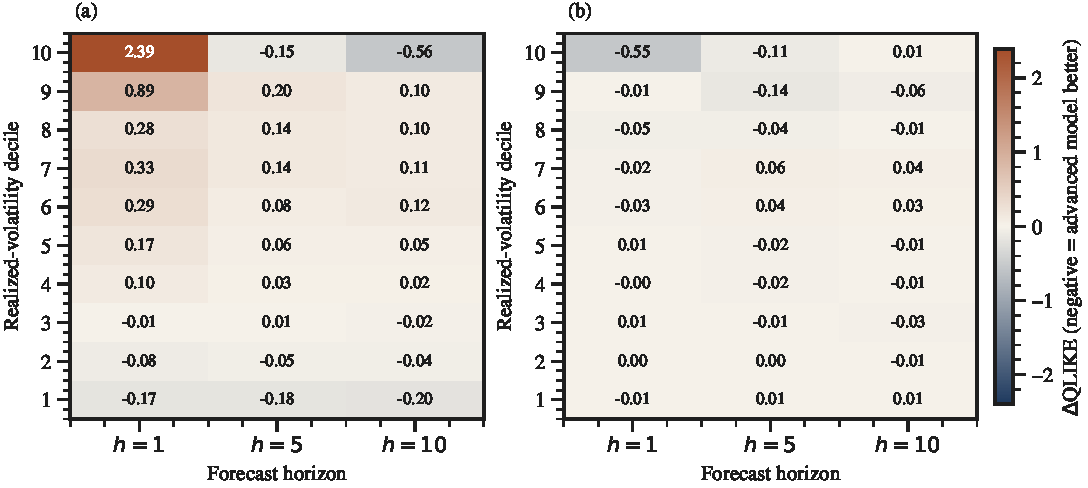
\includegraphics[width=0.96\textwidth]{figures/fig13_quantile_conditioned_delta.pdf}
\caption{Quantile-conditioned $\Delta$QLIKE surfaces. Panel (a) reports Wavelet-LightGBM minus HAR averaged across all indices in the full 2016--2025 package. Panel (b) reports Spillover-LGB minus Wavelet-LGB for the pooled DJIA and S\&P 500 spillover package. Negative values indicate that the more advanced model improves accuracy.}
\label{fig:quantile_conditioned_delta}
\end{figure}

Figure~\ref{fig:quantile_conditioned_delta} shows why the paper should not be read as a simple mean-rank comparison. Panel~(a) indicates that the multiscale model does not improve monotonically over HAR as realized volatility rises. Instead, its advantage is strongest in the calmest deciles and again in the most turbulent decile, while HAR remains strongest in the middle range where volatility is persistent but not yet severely stressed. This U-shaped pattern is economically interpretable. When the market is in a routine regime, short-horizon persistence remains hard to beat. When the market becomes extremely calm or clearly stressed, however, richer scale-specific information becomes more useful. Panel~(b) reveals a parallel result for spillover. The gain from adding peer-index wavelet features is concentrated in the upper volatility deciles, especially at \(h=1\) and \(h=5\), which is consistent with a state-dependent transmission mechanism rather than a uniform cross-market effect.

\begin{figure}[!t]
\centering
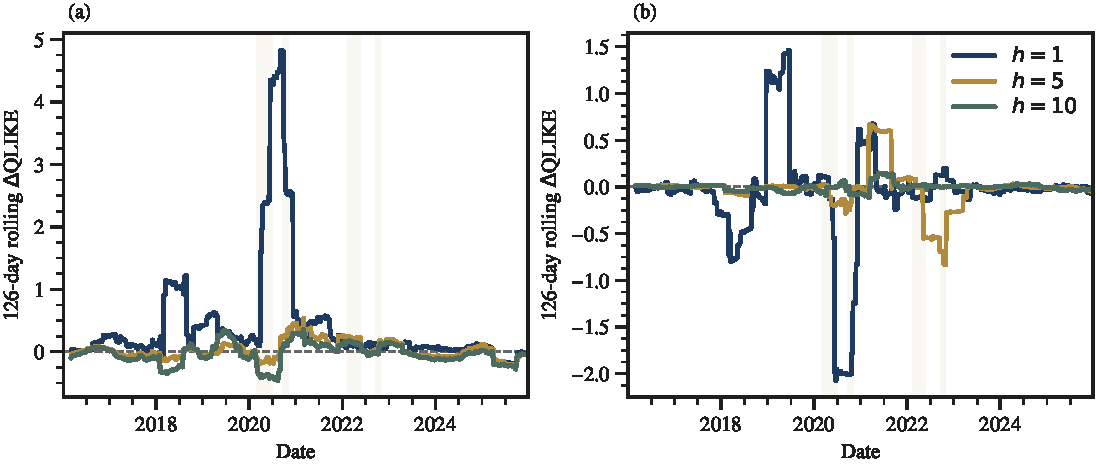
\includegraphics[width=0.96\textwidth]{figures/fig15_timevarying_gain_paths.pdf}
\caption{Time-varying gain paths based on 126-day rolling average $\Delta$QLIKE. Panel (a) reports Wavelet-LGB minus HAR averaged across all indices in the full 2016--2025 package. Panel (b) reports Spillover-LGB minus Wavelet-LGB for the pooled DJIA and S\&P 500 spillover package. Negative values indicate that the more advanced model improves accuracy. Shaded regions denote pooled top-decile VIX stress windows.}
\label{fig:timevarying_gain_paths}
\end{figure}

Figure~\ref{fig:timevarying_gain_paths} shows that the same pattern persists in calendar time. In the pooled 126-day rolling comparison, Wavelet-LGB stays below HAR in only \(8.1\%\) of the \(h=1\) windows, but this share rises to \(50.7\%\) at \(h=5\) and \(59.0\%\) at \(h=10\). The horizon effect is therefore not an artefact of full-sample averaging; it becomes more stable as the target moves away from the one-day persistence problem. Panel~(b) adds the spillover perspective: Spillover-LGB stays below the within-index wavelet model in \(66.8\%\), \(55.7\%\), and \(50.0\%\) of the broad-market rolling windows at \(h=1\), \(h=5\), and \(h=10\), respectively, with the clearest advantages clustered around the 2020 and 2022 stress windows. These diagnostics justify the central framing of the paper: the value of CMWSL is conditional, and those conditions align with economically meaningful market states.

\subsection{Main Forecasting Results: Strong Benchmark, Narrow Margins}

\begin{table}[!t]
\caption{Main regression QLIKE across indices and forecast horizons under the Rogers--Satchell target. Best, second-best, and third-best values within each index--horizon cell are marked by \best{bold shading}, \second{underline}, and \third{light shading}, respectively.}
\label{tab:main_regression}
\centering
\small
\setlength{\tabcolsep}{6pt}
\renewcommand{\arraystretch}{1.12}
\begin{tabular}{llccc}
\toprule
Index & Model & $h=1$ & $h=5$ & $h=10$ \\
\midrule
S\&P 500 & HAR & \best{-9.0316} & \best{-8.9372} & \second{-8.8682} \\
 & HV-22 & \second{-8.9405} & -8.8601 & -8.7836 \\
 & LightGBM & \third{-8.7386} & \second{-8.9022} & \best{-8.8749} \\
 & Wavelet-LightGBM & -8.7327 & \third{-8.8937} & \third{-8.8603} \\
\midrule
Nasdaq-100 & HAR & \best{-8.5635} & \third{-8.4940} & \third{-8.4316} \\
 & HV-22 & \second{-8.5049} & -8.4472 & -8.3873 \\
 & LightGBM & \third{-8.4476} & \best{-8.5125} & \second{-8.4621} \\
 & Wavelet-LightGBM & -8.3827 & \second{-8.5026} & \best{-8.4923} \\
\midrule
DJIA & HAR & \best{-9.0021} & \best{-8.9139} & \third{-8.8548} \\
 & HV-22 & \second{-8.9398} & \third{-8.8619} & -8.7869 \\
 & LightGBM & \third{-8.5186} & -8.8111 & \second{-8.8636} \\
 & Wavelet-LightGBM & -8.2222 & \second{-8.8649} & \best{-8.8934} \\
\bottomrule
\end{tabular}
\end{table}


\begin{figure}[!t]
\centering
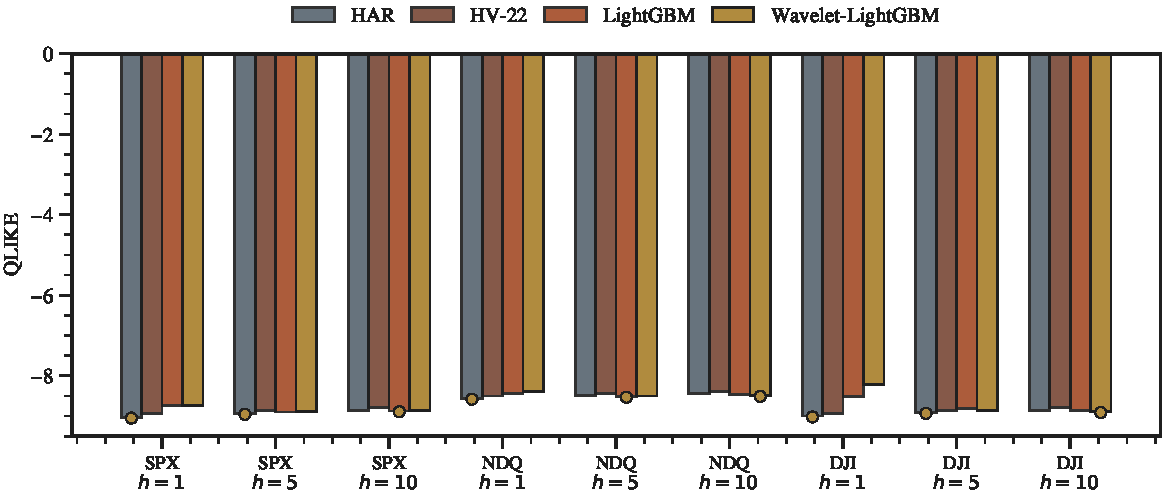
\includegraphics[width=0.98\textwidth]{figures/fig02_main_qlike_bars.pdf}
\caption{QLIKE across indices and forecast horizons in the main Rogers--Satchell specification. Lower values indicate better performance.}
\label{fig:main_qlike_bars}
\end{figure}

\begin{figure}[!t]
\centering
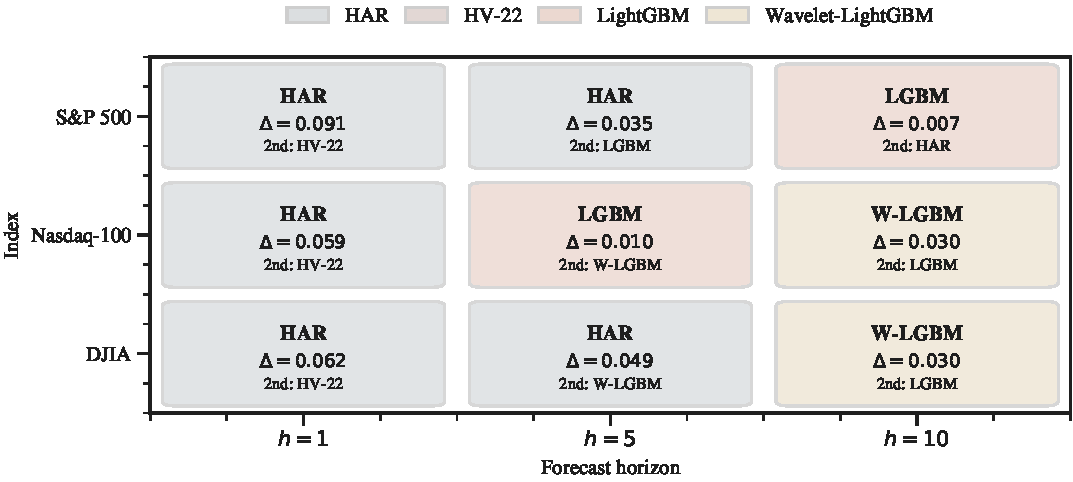
\includegraphics[width=0.98\textwidth]{figures/fig03_main_qlike_heatmap.pdf}
\caption{Winner-and-margin map for the main Rogers--Satchell specification. Each tile reports the winner and its QLIKE margin over the runner-up.}
\label{fig:main_qlike_heatmap}
\end{figure}

Table~\ref{tab:main_regression} and Figures~\ref{fig:main_qlike_bars}--\ref{fig:main_qlike_heatmap} establish the baseline difficulty of the forecasting problem. In the main Rogers--Satchell specification, HAR remains the best average model on QLIKE, with an average value of \(-8.789\), compared with \(-8.724\) for HV-22, \(-8.681\) for raw LightGBM, and \(-8.649\) for \textit{wavelet\_lightgbm}. This is a substantive result rather than a negative one. It confirms that daily stock-index volatility remains dominated by persistence, and that any paper claiming strong performance gains should be judged against that fact.

At the cell level, however, the picture is more nuanced. HAR wins five of the nine index--horizon contests, while LightGBM and \textit{wavelet\_lightgbm} each win two. The multiscale model is strongest for DJIA at \(h=10\) and Nasdaq-100 at \(h=10\), while raw LightGBM wins Nasdaq-100 at \(h=5\) and S\&P~500 at \(h=10\). Figure~\ref{fig:main_qlike_heatmap} is especially informative because it shows that several medium- and longer-horizon contests are narrow even when HAR remains the formal winner. The main sample should therefore be interpreted as showing two things simultaneously: short-horizon persistence is extremely hard to beat, but multiscale representation becomes meaningfully competitive once the horizon lengthens.

\subsection{Richer Public Information Strengthens the Multiscale Design}

\begin{table}[!t]
\caption{Average QLIKE across the main and robustness settings. Ranking is applied within each row.}
\label{tab:robustness_summary}
\centering
\small
\setlength{\tabcolsep}{6pt}
\renewcommand{\arraystretch}{1.12}
\begin{tabular}{lccc}
\toprule
Setting & HAR & LightGBM & Wavelet-LightGBM \\
\midrule
Main RS & \best{-8.7885} & \second{-8.6812} & \third{-8.6494} \\
Expanded Data & \best{-9.5949} & \third{-9.5641} & \second{-9.5704} \\
Parkinson & \third{-9.3019} & \second{-9.3091} & \best{-9.3143} \\
\bottomrule
\end{tabular}
\end{table}


\begin{figure}[!t]
\centering
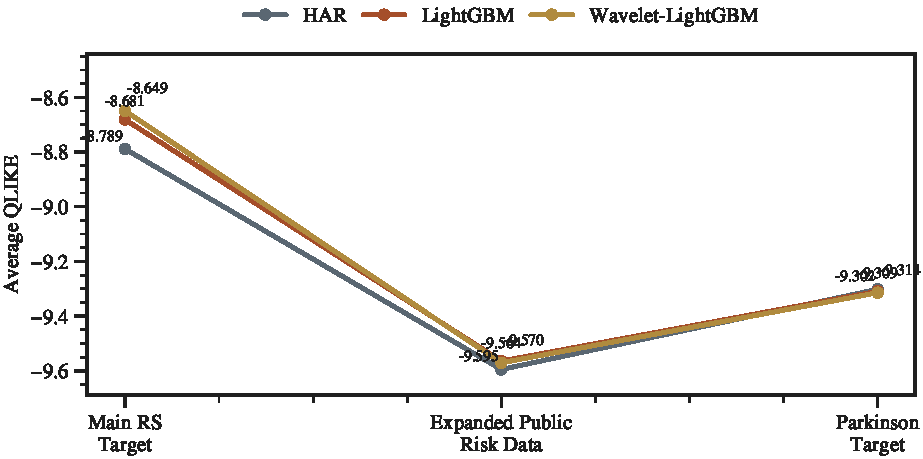
\includegraphics[width=0.94\textwidth]{figures/fig04_robustness_comparison.pdf}
\caption{Average QLIKE across the main and robustness settings. Lower values indicate better performance.}
\label{fig:robustness_comparison}
\end{figure}

\begin{figure}[!t]
\centering
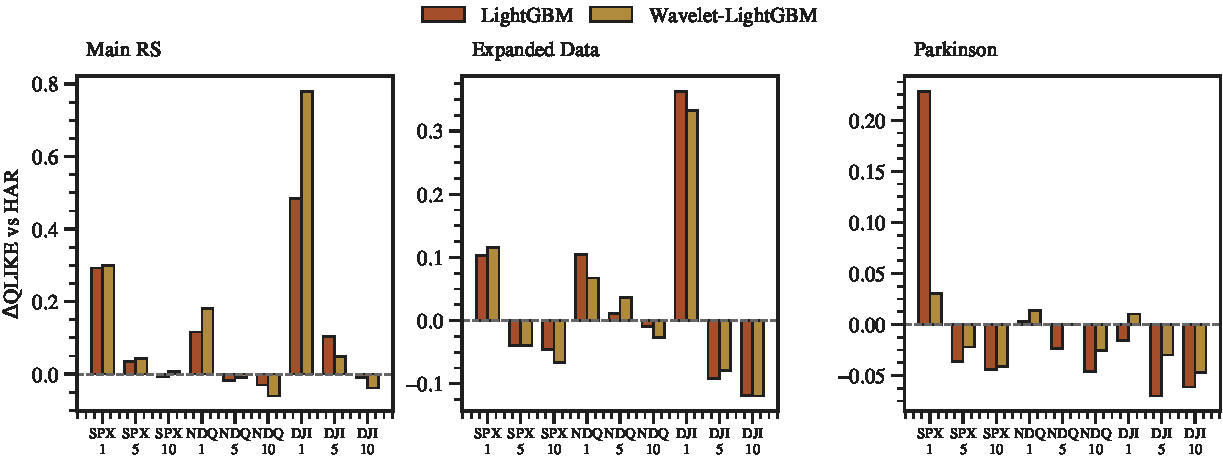
\includegraphics[width=0.94\textwidth]{figures/fig07_delta_vs_har.pdf}
\caption{Cell-level QLIKE differences relative to HAR. Negative values indicate that the nonlinear model outperforms HAR.}
\label{fig:delta_vs_har}
\end{figure}

The expanded public-information setting provides stronger support for CMWSL. After adding public credit-spread, policy-uncertainty, and volatility-term-structure variables, the average QLIKE of \textit{wavelet\_lightgbm} improves to \(-9.570\), much closer to HV-22 \((-9.618)\) and HAR \((-9.595)\). In this richer environment, the multiscale model wins four of the nine index--horizon cells, including DJIA at \(h=10\), Nasdaq-100 at \(h=10\), and S\&P~500 at both \(h=5\) and \(h=10\). This shift is central to the paper's interpretation. It suggests that the wavelet layer is not merely fitting noise in the main sample; it becomes more useful precisely when the public information set contains broader market-risk content that benefits from multiscale organization.

Figures~\ref{fig:robustness_comparison} and~\ref{fig:delta_vs_har} reinforce this interpretation. The comparison against HAR improves not only on average, but also in the cell-by-cell pattern. Appendix Figure~\ref{fig:forecast_panels_appendix} shows the same effect in time-series traces: isolated spikes still often favor HAR, but the wavelet-enhanced model tracks stress build-up and normalization more smoothly at \(h=5\) and \(h=10\). Appendix Figures~\ref{fig:multiscale_signal_heatmap_appendix} and~\ref{fig:block_contribution_heatmap_appendix} further indicate that the strongest associations with future volatility lie in longer-scale detail components and that macro-financial information becomes the most useful feature block once the public-information panel is expanded.

\subsection{Alternative Target and Risk-Warning Evidence}

The Parkinson robustness experiment sharpens the same message. Under this alternative OHLC target, \textit{wavelet\_lightgbm} achieves the best average QLIKE at \(-9.314\), slightly outperforming LightGBM \((-9.309)\) and HAR \((-9.302)\). The raw boosting model still wins five of the nine cells, so the result should not be overstated. But the average lead of the wavelet model is important because it indicates that CMWSL is more useful when the target itself contains richer range information than in the baseline Rogers--Satchell setting.

\begin{table}[!t]
\caption{Main warning results under the Rogers--Satchell target. PR-AUC is maximized and Brier score is minimized within each index--horizon cell.}
\label{tab:warning_results}
\centering
\small
\setlength{\tabcolsep}{5.2pt}
\renewcommand{\arraystretch}{1.12}
\begin{tabular}{llcccccc}
\toprule
Index & Model & PR$(1)$ & Brier$(1)$ & PR$(5)$ & Brier$(5)$ & PR$(10)$ & Brier$(10)$ \\
\midrule
S\&P 500 & Naive Threshold & \second{0.4895} & \best{0.0948} & \second{0.5041} & \best{0.0985} & \second{0.4474} & \best{0.1041} \\
 & Logistic-Raw & \best{0.5275} & \second{0.1327} & \best{0.5048} & \second{0.1271} & \best{0.5530} & \second{0.1143} \\
\midrule
Nasdaq-100 & Naive Threshold & \second{0.4652} & \best{0.1072} & \second{0.5141} & \best{0.1090} & \second{0.4496} & \best{0.1148} \\
 & Logistic-Raw & \best{0.5496} & \second{0.1418} & \best{0.5960} & \second{0.1258} & \best{0.4852} & \second{0.1399} \\
\midrule
DJIA & Naive Threshold & \second{0.4733} & \best{0.0954} & \second{0.4882} & \best{0.0972} & \best{0.4712} & \best{0.0998} \\
 & Logistic-Raw & \best{0.4900} & \second{0.1402} & \best{0.5782} & \second{0.1069} & \second{0.4672} & \second{0.1112} \\
\bottomrule
\end{tabular}
\end{table}


\begin{figure}[!t]
\centering
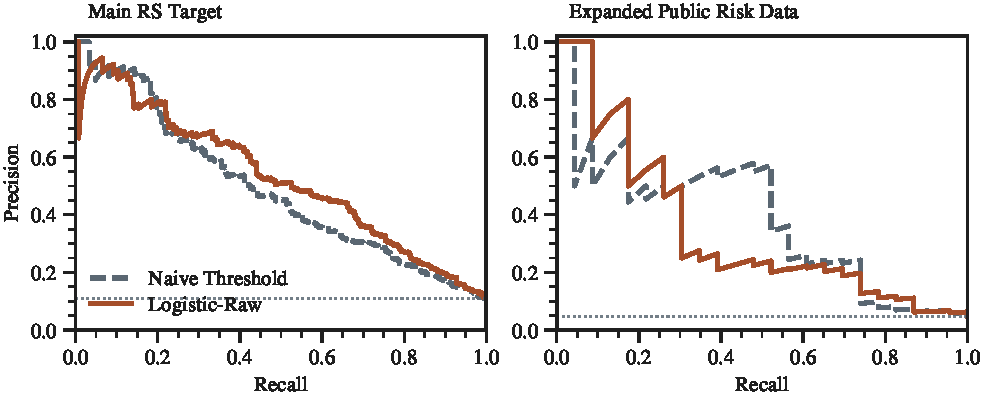
\includegraphics[width=0.94\textwidth]{figures/fig06_warning_pr_panels.pdf}
\caption{Precision--recall comparison for the warning task using the S\&P 500 at \(h=1\).}
\label{fig:warning_panels}
\end{figure}

\begin{figure}[!t]
\centering
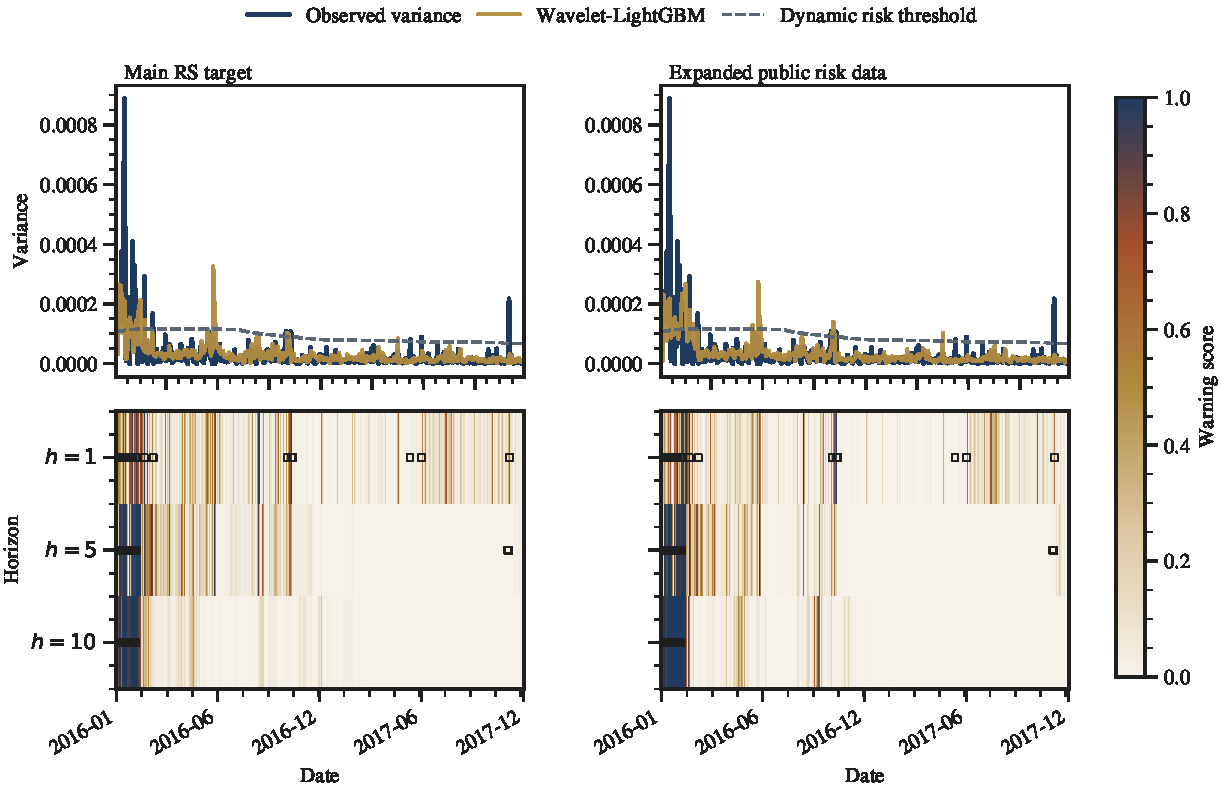
\includegraphics[width=0.94\textwidth]{figures/fig08_warning_score_distribution.pdf}
\caption{Event-aligned warning diagnostics for the S\&P 500 during the 2020 stress period.}
\label{fig:warning_score_distribution}
\end{figure}

\begin{table}[!t]
\caption{Event-based warning timing summary using a five-day pre-event detection window. Hit rate and median lead are maximized; false-alarm days per event are minimized within each horizon.}
\label{tab:warning_event_timing}
\centering
\footnotesize
\setlength{\tabcolsep}{4.6pt}
\renewcommand{\arraystretch}{1.12}
\begin{tabular}{llcccc}
\toprule
Horizon & Model & Hit rate & Median lead & FA / event & Events \\
\midrule
$h=1$ & Logistic-Raw & \best{0.821} & \best{5.000} & 5.149 & 460 \\
 & Naive-Threshold & 0.613 & 4.000 & \best{1.005} & 460 \\
\midrule
$h=5$ & Logistic-Raw & 0.597 & \best{5.000} & 16.558 & 134 \\
 & Naive-Threshold & \best{0.649} & 3.833 & \best{3.641} & 134 \\
\midrule
$h=10$ & Logistic-Raw & \best{0.602} & \best{5.000} & 37.330 & 81 \\
 & Naive-Threshold & 0.556 & 4.333 & \best{6.463} & 81 \\
\bottomrule
\end{tabular}
\end{table}


For the risk early-warning task, the clearest evidence comes from the interpretable logistic classifier estimated on raw market-risk features. In the main specification, \textit{logistic\_raw} reaches an average PR-AUC of \(0.528\), compared with \(0.478\) for the naive threshold rule, and also achieves a higher average ROC-AUC. In the expanded public-information setting, its PR-AUC rises further to \(0.593\), again the strongest result among the warning models. Under the Parkinson target, \textit{logistic\_raw} remains the top model on PR-AUC at \(0.559\). Figure~\ref{fig:warning_panels} makes this ranking visible in precision--recall space, while Figure~\ref{fig:warning_score_distribution} shows that elevated warning scores cluster around realized high-volatility episodes rather than appearing uniformly through time.

Table~\ref{tab:warning_event_timing} shows that warning quality should also be interpreted as a timing problem. Using a five-day pre-event detection window, \textit{logistic\_raw} detects a larger share of events than the threshold rule at \(h=1\) and \(h=10\) and also provides longer median lead times. The price is a higher alert burden, measured by false-alarm days per event. At \(h=5\), the threshold rule remains more economical and slightly stronger on hit rate. The practical implication is that the logistic warning model is more aggressive and earlier, whereas the threshold rule is sparser and more conservative. Appendix Figure~\ref{fig:warning_event_frontier_appendix} visualizes this operating frontier at the index--horizon level.

Full DM and CW benchmark-comparison tests are reported in Appendix Table~\ref{tab:significance_tests}. The overall message remains disciplined: there is no blanket nonlinear dominance, but there is clear evidence that incremental predictive content appears when the horizon lengthens, the information set broadens, or the market enters more stressed states.

\subsection{Cross-Index Spillover Ablation Results}
\label{subsec:results_spillover}

Table~\ref{tab:spillover_ablation} reports the full three-step ablation evidence over the 2016--2025 out-of-sample evaluation. This is the most direct test of the paper's novelty claim because it asks whether peer-index frequency-domain information adds value beyond within-index multiscale representation.

\begin{table}[!t]
\caption{Three-step ablation test results. Columns report mean QLIKE for each model, the
Diebold--Mariano statistic and p-value for Step~1 (HAR vs.\ Wavelet-LGB) and Step~2
(Wavelet-LGB vs.\ Spillover-LGB), and the Clark--West statistic and p-value for the
nested Step-2 comparison. DM tests are two-tailed with Newey-West HAC; CW test is
one-tailed (Ho:\ spillover carries no incremental information). Significance codes:
${}^{***}p<0.001$, ${}^{**}p<0.01$, ${}^{*}p<0.05$, ${}^{.}p<0.10$.
QLIKE convention: lower values indicate better forecasting accuracy.}
\label{tab:spillover_ablation}
\centering
\small
\setlength{\tabcolsep}{4pt}
\renewcommand{\arraystretch}{1.12}
\resizebox{\textwidth}{!}{%
\begin{tabular}{llccc  cc  cc  cc}
\toprule
 & & \multicolumn{3}{c}{Mean QLIKE} &
   \multicolumn{2}{c}{Step 1 DM} &
   \multicolumn{2}{c}{Step 2 DM} &
   \multicolumn{2}{c}{Step 2 CW (nested)} \\
\cmidrule(lr){3-5}\cmidrule(lr){6-7}\cmidrule(lr){8-9}\cmidrule(lr){10-11}
Index & $h$ & HAR & Wav-LGB & Spill-LGB &
  $t_{\!DM}$ & $p$ &
  $t_{\!DM}$ & $p$ &
  $t_{\!CW}$ & $p$ \\
\midrule
DJIA & $h=1$ & $-9.0021$ & $-8.1817$ & $-8.2476$ & $-3.666$ & $0.0002^{***}$ & $0.317$ & $0.7515$ & $1.749$ & $0.0401^{*}$ \\
 & $h=5$ & $-8.9139$ & $-8.6564$ & $-8.7303$ & $-2.356$ & $0.0185^{*}$ & $1.427$ & $0.1536$ & $2.613$ & $0.0045^{**}$ \\
 & $h=10$ & $-8.8548$ & $-8.9037$ & $-8.8932$ & $1.522$ & $0.1280$ & $-0.812$ & $0.4166$ & $1.394$ & $0.0816^{.}$ \\
\midrule
Nasdaq-100 & $h=1$ & $-8.5635$ & $-8.2771$ & $-8.2892$ & $-4.881$ & $<0.0001^{***}$ & $0.207$ & $0.8363$ & $0.293$ & $0.3847$ \\
 & $h=5$ & $-8.4940$ & $-8.5154$ & $-8.5027$ & $1.308$ & $0.1909$ & $-0.983$ & $0.3256$ & $-1.521$ & $0.9358$ \\
 & $h=10$ & $-8.4316$ & $-8.5149$ & $-8.5103$ & $3.417$ & $0.0006^{***}$ & $-0.625$ & $0.5318$ & $0.977$ & $0.1644$ \\
\midrule
S\&P~500 & $h=1$ & $-9.0316$ & $-8.8211$ & $-8.8841$ & $-2.637$ & $0.0084^{**}$ & $1.353$ & $0.1761$ & $2.077$ & $0.0189^{*}$ \\
 & $h=5$ & $-8.9372$ & $-8.8741$ & $-8.8444$ & $-1.046$ & $0.2957$ & $-0.548$ & $0.5838$ & $1.945$ & $0.0259^{*}$ \\
 & $h=10$ & $-8.8682$ & $-8.8970$ & $-8.9141$ & $0.772$ & $0.4402$ & $1.199$ & $0.2307$ & $4.827$ & $<0.0001^{***}$ \\
\bottomrule
\end{tabular}
}
\end{table}


\begin{figure}[!t]
\centering
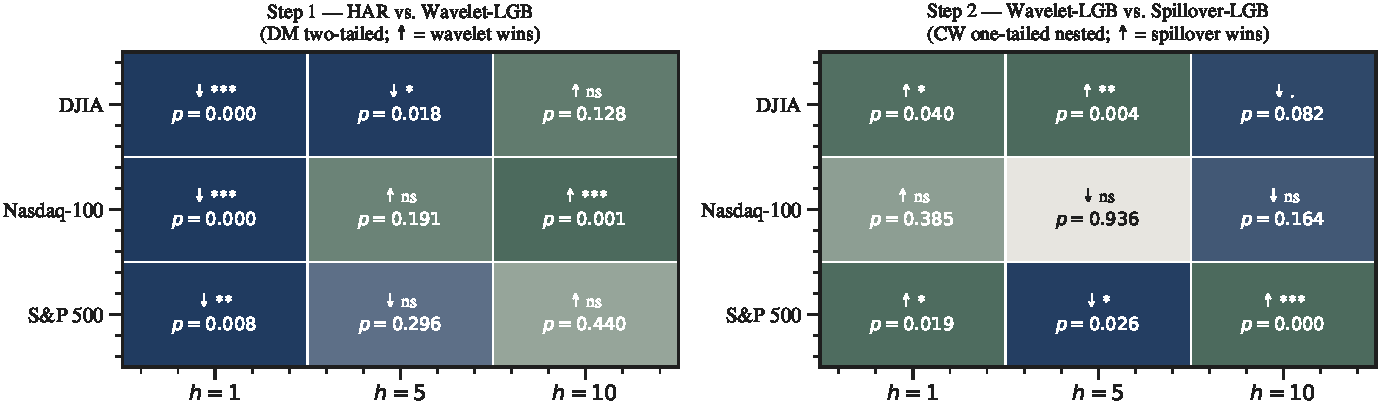
\includegraphics[width=0.94\textwidth]{figures/fig_spillover_cw_heatmap.pdf}
\caption{Statistical evidence heatmap for each ablation step.
  Left: Diebold--Mariano two-tailed test for Step~1 (HAR vs.\ Wavelet-LGB).
  Right: Clark--West one-tailed test for Step~2 (Wavelet-LGB vs.\ Spillover-LGB).
  Teal tones indicate that the advanced model wins at the stated significance level;
  navy tones indicate the simpler model wins.
  Colour intensity scales with $1-p$.}
\label{fig:spillover_cw_heatmap}
\end{figure}

\begin{figure}[!t]
\centering
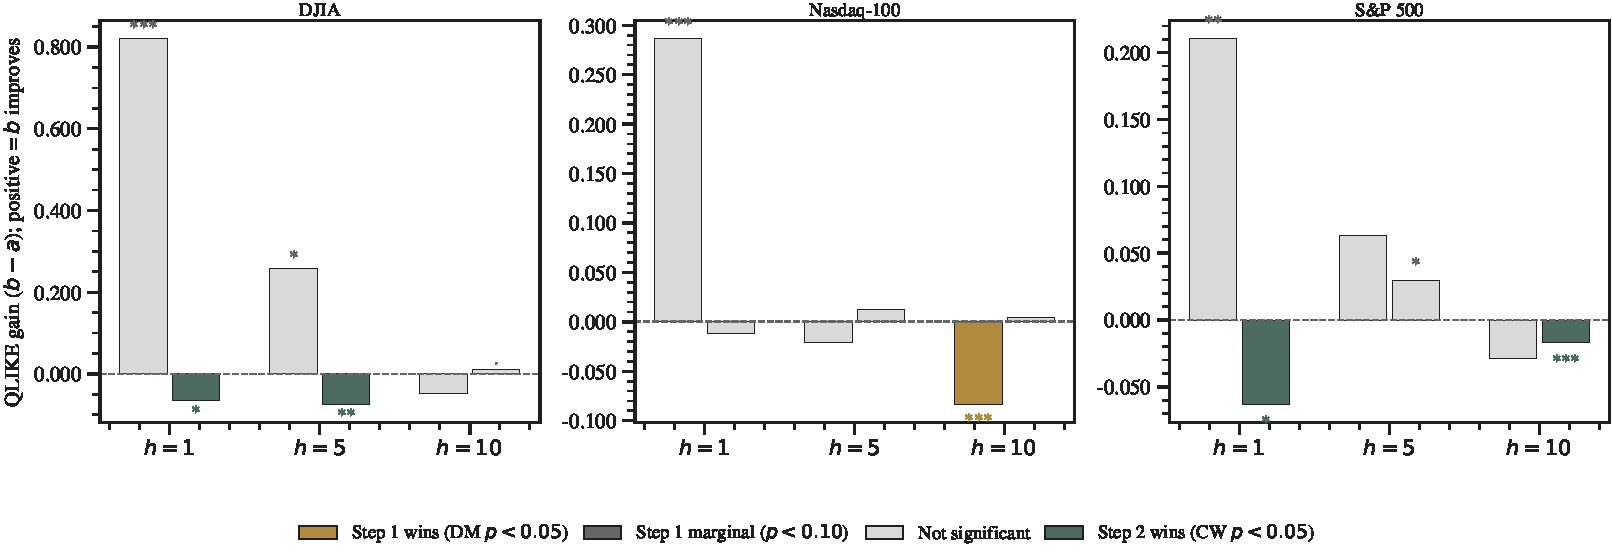
\includegraphics[width=0.94\textwidth]{figures/fig_spillover_gain_ladder.pdf}
\caption{QLIKE gain ladder per index.
  Each panel shows the incremental QLIKE gain (positive = improvement over baseline)
  for Step~1 (amber bars when DM-significant, light grey otherwise) and
  Step~2 (teal bars when CW-significant, light grey otherwise).
  Significance codes: ${}^{***}p<0.001$, ${}^{**}p<0.01$, ${}^{*}p<0.05$, ${}^{.}p<0.10$.}
\label{fig:spillover_gain_ladder}
\end{figure}

\paragraph{Step~1: HAR versus within-index wavelet representation.}
The first ablation step shows that within-index wavelet features add value selectively rather than uniformly. For DJIA, HAR significantly outperforms Wavelet-LGB at \(h=1\) (DM \(t=-3.67\), \(p<0.001\)) and \(h=5\) (\(p=0.019\)), confirming that short-run persistence dominates for this broad, price-weighted index. The relative advantage narrows at \(h=10\), where Wavelet-LGB posts a slightly better QLIKE, though not significantly so. For Nasdaq-100, HAR dominates strongly at \(h=1\) (DM \(t=-4.88\), \(p<0.001\)), but the relation reverses at \(h=10\) (\(p=0.001\)), indicating richer long-horizon multiscale structure in the technology-heavy index. For S\&P~500, HAR wins significantly at \(h=1\), while the medium- and long-horizon cells are statistically inconclusive. Step~1 therefore supports the first part of the paper's argument: wavelet representation is most useful when the problem moves away from the one-day persistence regime.

\paragraph{Step~2: within-index wavelet versus spillover-augmented wavelet.}
The second ablation step is the core test of the Cross-Index Wavelet Spillover Hypothesis. The two-sided DM test does not reach \(p<0.05\) in any of the nine cells, which is not surprising in a nested setting where the larger model pays an estimation-noise penalty. The CW test, which is specifically designed for nested comparisons, paints a more informative picture.

Five of the nine cells are significant at \(p<0.05\) under CW. DJIA shows significant gains at \(h=1\) (CW \(t=1.75\), \(p=0.040\)) and \(h=5\) (CW \(t=2.61\), \(p=0.005\)). S\&P~500 shows significant gains at \(h=1\) (\(p=0.019\)), \(h=5\) (\(p=0.026\)), and most strongly at \(h=10\) (CW \(t=4.83\), \(p<0.001\)). The S\&P~500 \(h=10\) cell is the clearest positive result in the article: peer-index d2/d3 wavelet energy provides information about future broad-market volatility that is not already contained in the target index's own persistence and multiscale history.

Nasdaq-100 behaves differently. None of its three cells is significant under CW, and the \(h=5\) cell even shows a negative CW statistic. This absence of spillover response is informative in its own right. It suggests that the volatility dynamics of a technology-concentrated index occupy a different frequency-domain regime from those of the broad-market indices used as peers. The same weekly-to-biweekly peer-market channels that help forecast DJIA and S\&P~500 do not transfer cleanly to Nasdaq-100.

The regime-conditioned evidence in Appendix Table~\ref{tab:spillover_regime} sharpens this interpretation. For the pooled DJIA and S\&P~500 sample, spillover gains are strongest in recession and high-VIX windows at \(h=1\) and \(h=5\). Combined with Figures~\ref{fig:quantile_conditioned_delta} and~\ref{fig:timevarying_gain_paths}, the result supports a clear interpretation: peer-index wavelet information is most useful when broad-market stress is elevated, synchronized, and still unfolding.

\paragraph{Why DM and CW differ.}
The divergence between DM and CW is not contradictory. DM tests realized loss differences directly and does not correct for the attenuation induced by estimating additional regressors in the larger model. CW adds the usual nested-model adjustment term \((\hat y_{1,t}-\hat y_{2,t})^2\), which raises power when the larger model contains real but noisy incremental information \cite{clark2007nested}. In the present setting, the pattern of positive QLIKE gains combined with CW significance indicates that the spillover features contain useful predictive signal, even though that signal is modest and partially offset by estimation noise in finite rolling samples.

\paragraph{Takeaway from the ablation.}
The spillover ladder establishes three regularities. HAR remains the dominant short-horizon benchmark. Within-index wavelet representation adds value selectively, mainly at longer horizons. Cross-index d2/d3 spillover features provide statistically significant incremental information for DJIA and S\&P~500 at multiple horizons, with the S\&P~500 \(h=10\) cell providing the strongest evidence. This is the most novel result of the paper because it isolates a specific type of cross-market information that matters precisely where time-domain persistence becomes less sufficient.

\subsection{Interpretability and Deep-Learning Benchmarking}
\label{subsec:results_shap}

To examine whether the gains of CMWSL are driven by economically meaningful inputs rather than by opaque tree interactions, we compute SHAP values \cite{lundberg2017shap} for a full-window \textit{wavelet\_lightgbm} model fitted at the start of the test period for the S\&P~500 index at both $h=1$ and $h=5$.

\begin{figure}[!t]
\centering
\subfloat[$h=1$: persistence and short-run signals dominate; wavelet features appear further down.\label{fig:shap_bar_h1}]{%
  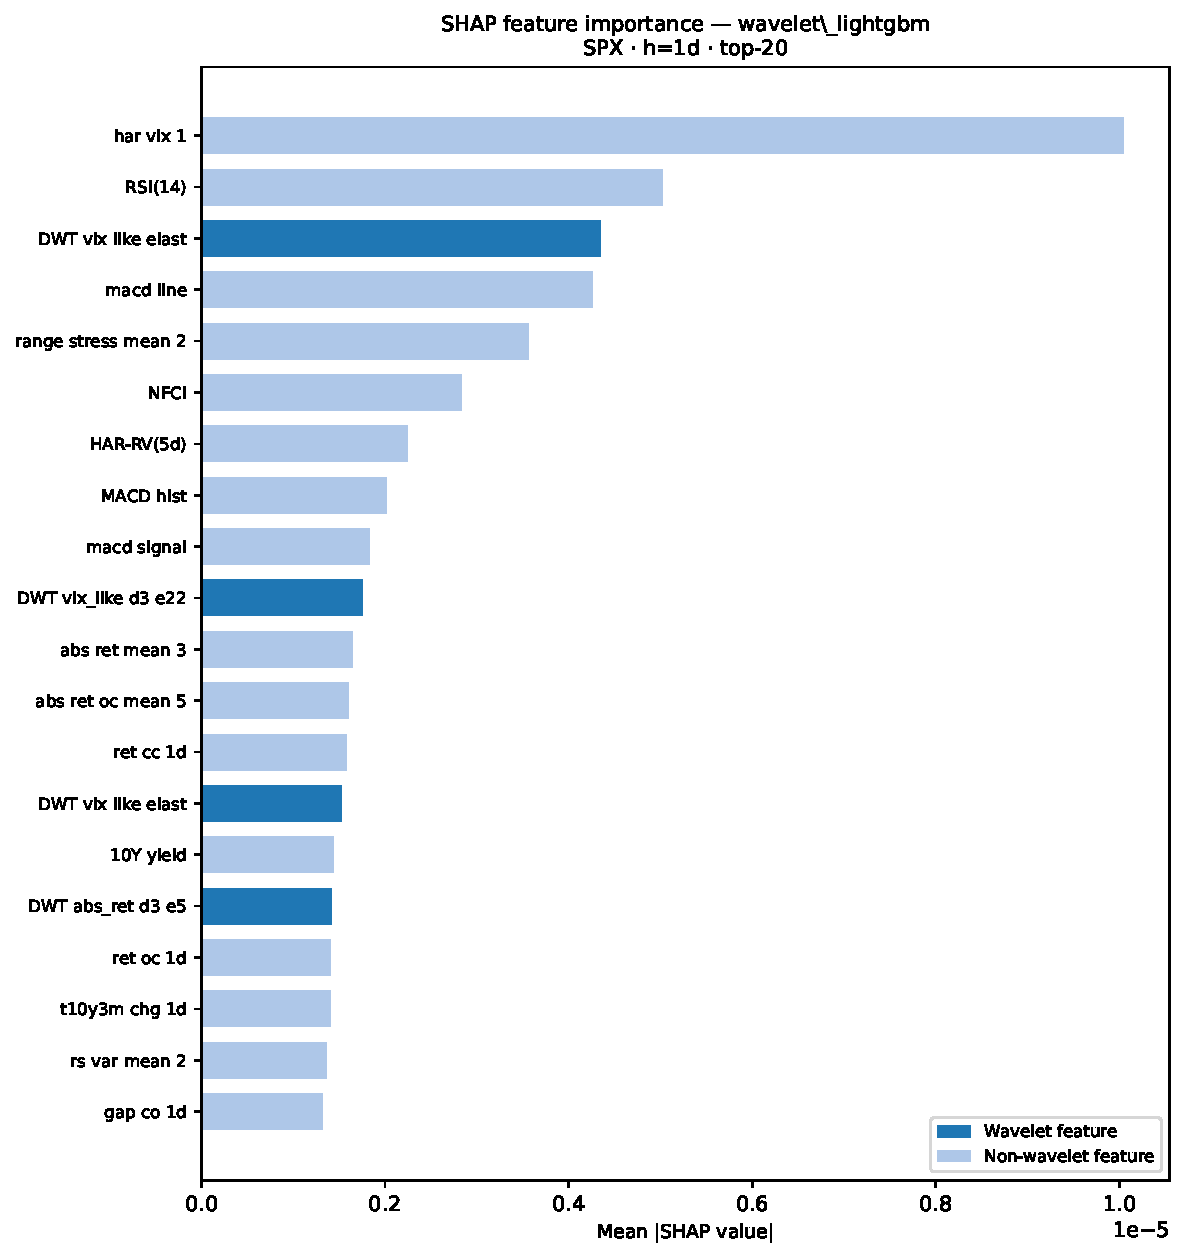
\includegraphics[width=0.47\textwidth]{figures/shap_bar_spx_h1.pdf}}
\hfill
\subfloat[$h=5$: wavelet energy at d2/d3 scales rises sharply in the ranking.\label{fig:shap_bar_h5}]{%
  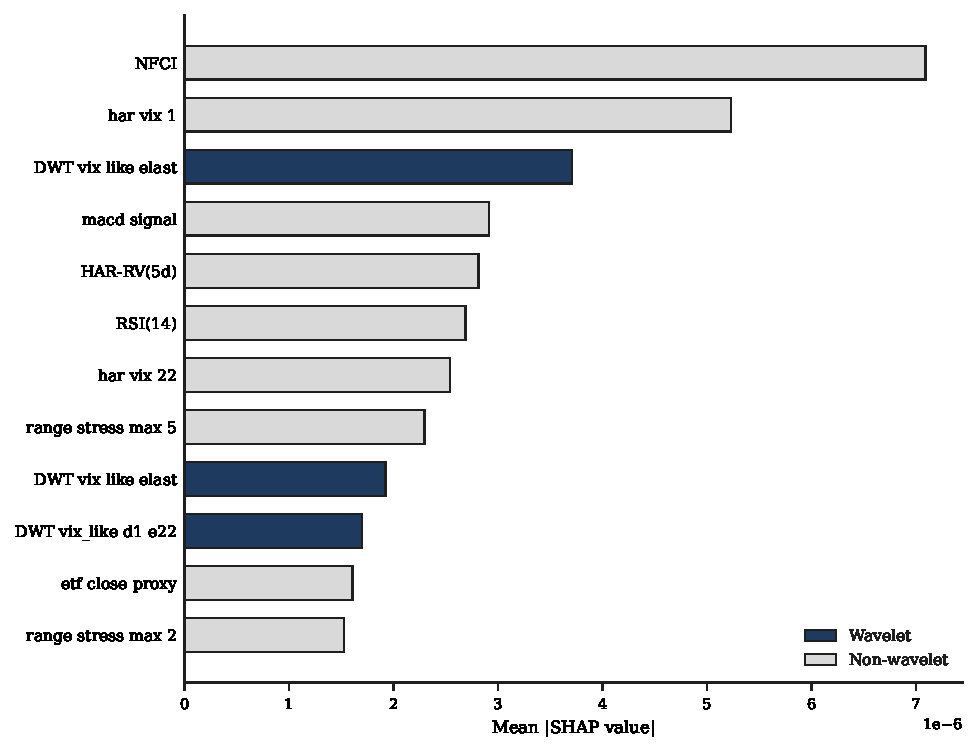
\includegraphics[width=0.47\textwidth]{figures/shap_bar_spx_h5.pdf}}
\caption{Horizon-dependent SHAP feature attribution (top-12 mean absolute values) for \textit{wavelet\_lightgbm} (S\&P~500). Navy bars denote wavelet features; grey bars denote non-wavelet features. The shift from $h=1$ to $h=5$ confirms that medium-scale frequency-domain information adds value selectively as the forecast horizon lengthens---consistent with the quantile-conditioned and rolling-window evidence in Figures~\ref{fig:quantile_conditioned_delta} and~\ref{fig:timevarying_gain_paths}.}
\label{fig:shap_horizon_comparison}
\end{figure}

\begin{figure}[!t]
\centering
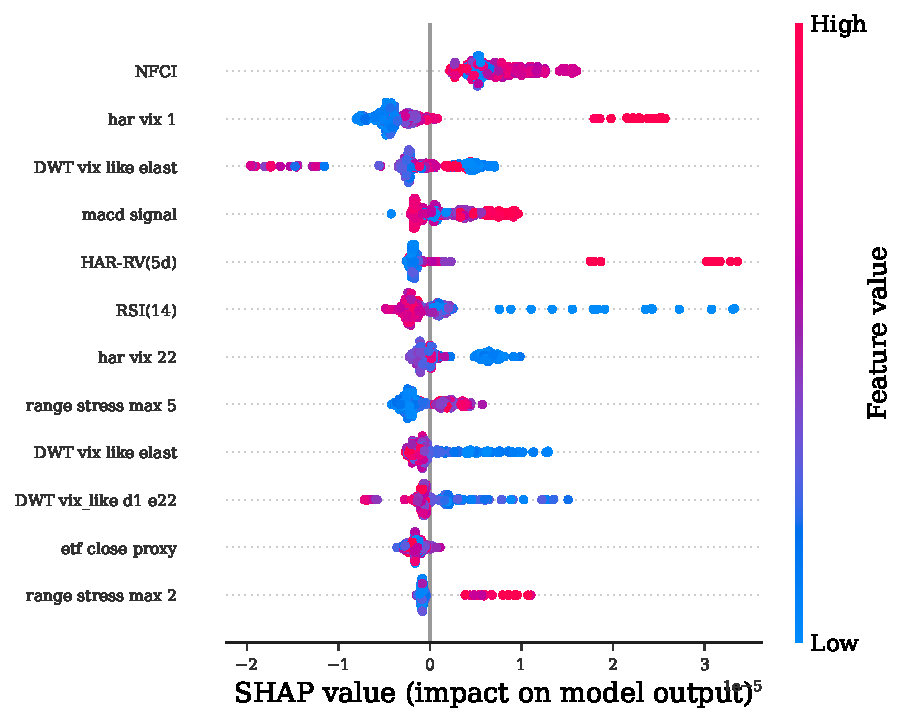
\includegraphics[width=0.60\textwidth]{figures/shap_beeswarm_spx_h5.pdf}
\caption{SHAP beeswarm for \textit{wavelet\_lightgbm} (S\&P~500, $h=5$). Each point is one observation; colour encodes the feature value. SWT energy features at the d2/d3 decomposition levels rank among the most influential predictors, and high energy values consistently produce positive SHAP contributions, confirming that medium-scale frequency-domain volatility drives upward forecast revisions.}
\label{fig:shap}
\end{figure}

Figure~\ref{fig:shap_horizon_comparison} documents the horizon-dependent shift in feature importance. At $h=1$, HAR persistence lags and short-run technical signals such as MACD and ATR dominate the ranking, consistent with a regime where next-day volatility is primarily determined by the recent level and trajectory of the series. At $h=5$, wavelet energy variables at the d2 and d3 scales of the VIX-related and Rogers--Satchell input series move to the top of the ranking, while the relative importance of raw persistence lags declines. This transition mirrors the pattern documented in Figures~\ref{fig:quantile_conditioned_delta} and~\ref{fig:timevarying_gain_paths}, and directly supports the paper's central interpretation that medium-scale frequency-domain structure becomes decision-relevant precisely as the forecast horizon extends into the range most useful for portfolio risk monitoring.

\subsection{LSTM Baseline Comparison}
\label{subsec:results_dl}

To test whether the performance of \textit{wavelet\_lightgbm} reflects feature quality rather than only model flexibility, we include a compact LSTM baseline evaluated under the same 1260-day rolling protocol. The LSTM is trained on the three HAR inputs, uses 16 hidden units with chronological early stopping, and targets the same log1p-transformed realized variance as the tree-based models. This HAR-LSTM specification asks whether a neural sequence model can extract gains from the standard persistence feature set without the wavelet layer.

\begin{table}[!t]
\caption{QLIKE comparison of benchmark models and the HAR-LSTM deep-learning
baseline under the same 1260-day rolling walk-forward protocol.
The LSTM is trained on the three HAR features (1-, 5-, and 22-day realized
variance) with 16 hidden units and chronological early stopping.
Best value per index--horizon cell is \best{bold-shaded}; second-best is \second{underlined}.}
\label{tab:dl_comparison}
\centering
\small
\setlength{\tabcolsep}{5pt}
\renewcommand{\arraystretch}{1.10}
\begin{tabular}{llccc}
\toprule
Index & Model & $h=1$ & $h=5$ & $h=10$ \\
\midrule
S\&P 500 & HAR & \best{0.5204} & \best{0.3168} & \second{0.3085} \\
  & HV-22 & 0.6122 & 0.3939 & 0.3932 \\
  & LightGBM & 0.8149 & \second{0.3518} & \best{0.3019} \\
  & \textit{wavelet\_lightgbm} & 0.8210 & 0.3603 & 0.3165 \\
\cmidrule(lr){2-5}
  & LSTM & \second{0.6072} & 0.3946 & 0.3510 \\
\midrule
Nasdaq-100 & HAR & \best{0.4798} & 0.2763 & 0.2733 \\
  & HV-22 & 0.5386 & 0.3231 & 0.3176 \\
  & LightGBM & 0.5955 & \best{0.2578} & \second{0.2428} \\
  & \textit{wavelet\_lightgbm} & 0.6607 & \second{0.2677} & \best{0.2126} \\
\cmidrule(lr){2-5}
  & LSTM & \second{0.5176} & 0.3097 & 0.2910 \\
\midrule
DJIA & HAR & \best{0.5169} & \best{0.3144} & 0.3048 \\
  & HV-22 & \second{0.5795} & 0.3665 & 0.3727 \\
  & LightGBM & 1.0023 & 0.4173 & \second{0.2960} \\
  & \textit{wavelet\_lightgbm} & 1.3000 & \second{0.3634} & \best{0.2662} \\
\cmidrule(lr){2-5}
  & LSTM & 0.5957 & 0.3653 & 0.3430 \\
\midrule
\bottomrule
\end{tabular}
\end{table}

Table~\ref{tab:dl_comparison} shows that the LSTM is broadly comparable to HAR at \(h=1\) but remains behind \textit{wavelet\_lightgbm} at \(h\ge 5\), where the multiscale feature advantage is most pronounced. This is important for the paper's interpretation. It indicates that the main contribution of CMWSL is not simply ``nonlinearity''. Rather, it is the design of a causal multiscale and spillover-aware feature space that can then be learned efficiently by a well-calibrated tree model.
